\documentclass[10pt,a4paper]{ujarticle}
\usepackage{amsmath}
\usepackage{amsfonts}
\usepackage{amssymb}
\usepackage{amsthm}
\usepackage{bm}
\usepackage{url}
\usepackage{comment}
\usepackage[dvipdfmx]{graphicx}
\usepackage{tikz}
\usetikzlibrary{arrows.meta}
\usepackage[top=30truemm,bottom=30truemm,left=25truemm,right=25truemm]{geometry}

\theoremstyle{definition}

\newtheorem{theorem}{定理}
\newtheorem{lemma}{補題}
\newtheorem{definition}{定義}
\newtheorem{remark}{注意}
\renewcommand{\proofname}{証明}

\usepackage{listings}

\lstset{basicstyle=\small\ttfamily}

\newcommand{\Npos}{\mathbb{N}_{\ge 1}}
\newcommand{\Mink}{\mathbin{+_{\mathrm M}}}
\newcommand{\length}[1]{\lvert #1\rvert}
\let\lean\path

\renewcommand{\labelenumi}{(\arabic{enumi})}

\author{山田 航輝}
\title{Scheckerの証明について}

\begin{document}
\maketitle

\begin{abstract}
本稿では，Schecker\cite{schecker}による $[\sqrt{21}, \infty) \subset M$の証明を検証した
\verb|schecker_proof_1.ipynb|および\verb|schecker_proof_2.ipynb|
の内容および妥当性について解説する．
\end{abstract}

\section{準備}
\begin{definition}
  \label{def:lagrange-spectrum}
  $A=(a_n)_{n\in\mathbb Z}\in\mathbb{N}^{\mathbb Z}$ と $i\in\mathbb Z$ に対して
  \[
    \lambda_i(A)
    =[a_i;a_{i+1},a_{i+2},\ldots]
     +[0;a_{i-1},a_{i-2},\ldots]
  \]
  とおく．そして
  \[
  l(A) = \limsup_{i\to \infty} \lambda_i(A), \quad m(A) = \sup_{i\in \mathbb{Z}} \lambda_i(A)
  \]
  とする．
  
  また，
    $N\in\mathbb{N}$ に対して
    \[
      C(N)=
      \left\{
        [0;a_1,a_2,\ldots]:1\le a_i\le N\quad(i\ge1)
      \right\}
    \]
    とおく．
\end{definition}

続いて，Scheckerの論文で定義されている概念を列挙する．
\begin{definition}
  \[
  \theta_i = \begin{cases}
    [0; \overline{1, 2}] \quad i : odd \\
    [0; \overline{2, 1}] \quad i : even
  \end{cases}, \quad 
  \eta_i = \begin{cases}
    [0; \overline{1, 3}] \quad i : odd \\
    [0; \overline{3, 1}] \quad i : even
  \end{cases},
  \]
  とおく．また，
  \[
  \mathcal{B}_{h,k} = \{ (a_i)_{-h \le i \le k} : a_i\in \mathbb{N}, 1\le a_i \le 4 \}
  \]
  とし，$A = (a_i) \in \mathcal{B}_{h,k}$について，$A$のT区間を以下のように定める:

  左端が
  \begin{align*}
    \min \{[0; a_{-1},\cdots , a_{-h} + \eta_h] + [0; a_1,\cdots , a_{k} + \theta_k],\\
    [0; a_{-1},\cdots , a_{-h} + \theta_h] + [0; a_1,\cdots , a_{k} + \eta_k] \}
  \end{align*}

  右端が
  \begin{align*}
    \max \{[0; a_{-1},\cdots , a_{-h} + \eta_{h + 1}] + [0; a_1,\cdots , a_k + \theta_{k + 1}],\\
    [0; a_{-1},\cdots , a_{-h} + \theta_{h + 1}] + [0; a_1,\cdots , a_{k} + \eta_{k + 1}] \}
  \end{align*}
  となる閉区間．

  これを$I(A)$とか，$I(a_{-1},\cdots, a_{-h} | a_1, \cdots a_k)$とかく．

  $v(A)$を
  \[
  v(A) = \left| \frac{[0; a_1,\cdots, a_k + \eta_1] - [0; a_1,\cdots, a_k + \eta_2]}{[0; a_{-1},\cdots, a_{-h} + \eta_1] - [0; a_{-1},\cdots, a_{-h} + \eta_2]}\right|
  \]
  と定め，これをT比と呼ぶ．

  $I(A)$が許容的であるとは，\begin{enumerate}
    \item $h \ge 2$ または$a_{-1} \ge 2$
    \item $k \ge 2$ または$a_1 \ge 2$
    \item $\frac{5}{17} \le v(A) \le \frac{17}{5}$
  \end{enumerate}
  が成立することである．

  $B = (b_i) \in \mathcal{B}_{h',k'}$が$A = (a_i) \in \mathcal{B}_{h,k}$の後続であるとは，
  \begin{enumerate}
    \item $k'\ge k, h' \ge h , k' + h' > k + h$
    \item $b_i = a_i$ $(-h\le i \le k)$
  \end{enumerate}
  が成立すること．さらに$1 \le b_i \le m$ $(-h' \le i < -h,\ k < i \le k')$が成立するとき，$m$-後続であるという．
\end{definition}

\section{\texttt{schecker\_proof\_1.ipynb}と主結果の証明}
次の補題はScheckerの結果全体を支える要石である．
\begin{lemma}
  \label{Lem1}
  許容的T区間は，許容的$3-$後続によって被覆される
\end{lemma}
ここから，次の定理を導くことができる
\begin{theorem}
  \label{Satz1}
  $A = (a_i)\in \mathcal{B}_{h,k}$とし，$I(A)$は許容的とする．このとき，$t\in I(A)$とする．$r, s\in C(3)$によって
  \[
  t = [0; a_{-1},\cdots, a_{-h} + r] + [0; a_{1},\cdots, a_{k} + s]
  \]
  と表せる．
\end{theorem}
\begin{proof}
  補題$\ref{Lem1}$より，$I(A)$は許容的$3$後続たちに被覆され，それらの許容的$3$後続たちもまた許容的な$3$後続たちに被覆される．

  ここから，単調非減少な添え字の列$(\nu_i), (\mu_i)$と，自然数列$(u_i), (w_i)$があって，$\nu_{i + 1} + \mu_{i + 1} > \nu_i + \mu_i$かつ，各$i$について
  $I(\sim u_1,\cdots, u_{\nu_i} | \sim w_1,\cdots, w_{\mu_i})$が$t$を含む$I(A)$の許容的$3$後続になる．

  一般性を失わず，$\nu_1 < \nu_2 < \cdots $としてよく，許容性から$\mu_i$も非有界である（負方向だけが極端に大きくなると，$v(A)$の定義の分母が小さくなり，
  したがって$v(A)$が，許容的になるには大きくなりすぎてしまう）．

  そして
  \[
  r = [0; u_1, u_2,\cdots], \quad s = [0; w_1,w_2,\cdots]
  \]
  とすれば，$r, s \in C(3)$で，
  \[
  t = [0; a_{-1},\cdots, a_{-h} + r] + [0; a_1,\cdots,a_k + s]
  \]
  となる．
\end{proof}

定理\ref{Satz1}により，$I(A)$が許容的となる$A\in \mathcal{B}_{h,k}$をもとに$M$に含まれる区間を次のように作れる（ことがある）．

と表せるのだから，$a_0$を適当に定め，
\[
\{(b_i) \in \mathbb{N}^\mathbb{Z} : a_i = b_i (-h \le i \le k ), 1\le b_i\le 3 (i < -h, k< i )\}
\]に属する両側無限列の$i\neq 0$での$\lambda_i$の値の上限を$\Lambda$とすれば，$[\Lambda,\infty) \cap (a_0 + I(A))\subset M$となる．
実際$t\in [\Lambda,\infty) \cap (a_0 + I(A))$とすると，
$t\in (a_0 + I(A))$だから，定理\ref{Satz1}により，$r, s\in C(3)$によって
\[
t = a_0 + [0; a_{-1},\cdots, a_{-h} + r] + [0; a_{1},\cdots, a_{k} + s]
\]
と表せる．$r = [0; b_1, b_2, \cdots], s = [0; c_1, c_2, \cdots]$とおき，
\[
B = (\cdots, b_2, b_1, a_{-h}, \cdots a_{-1}, a_0, a_1, \cdots a_k, c_1, c_2, \cdots)
\]とすることで，$\lambda_0(B) = t$となるが，
$\Lambda \le t$だから，$i\neq 0$について$\lambda_i(B) \le \lambda_0(B) = t$が分かる．つまり
\[
m(B) = \lambda_0(B) = t
\] 
となり$t\in M$が分かる．

\subsection{$M$に含まれる区間の構成}

\verb|schecker_proof_1.ipynb|の函数\verb|max_value_of_lambda_i|は，この$\Lambda$の算出を行っている．
具体的には．与えられた$A\in \mathcal{B}_{h,k}$（\verb|negative_side|，\verb|positive_side|，\verb|a_0|，に分けて入力される）に対して，
まず$-h \le i \le k(i\neq 0)$における$\lambda_i$の値としてありうる最大値を\verb|max_value_of_lambda|を使って算出し
（これは偶奇に合わせて$1,3$または$3,1$の繰り返しで延長するだけ），上限の候補リスト\verb|max_values|に追加する．
次に$i < -h$または$k < i$での$\lambda_i$の値の上限を算出しなくてはならないが，これは$\sqrt{21}$の可能性だけ考慮すれば十分である．実際，$A$を$1, 3$の繰り返しで延長したものを$B$とすると，
\[
\limsup_{i\to\infty}\lambda_i (B) = 3 + [0;\overline{1,3}] + [0;\overline{1,3}] = \sqrt{21}
\]
であるから，$\sqrt{21}$以上であることはすぐに分かる．

反対側も同様であるから，$k < i$として，$A$を$1,2,3$で延長した$\tilde{A}$について，$\lambda_i$の値を考える．
\[
\lambda_i(\tilde{A}) = a_i + [0;a_{i-1},\cdots] +  [0;a_{i+1},\cdots]\le 3 + [0;a_{i-1},\cdots,] + [0;\overline{1,3}]
\]
となることが分かる．ここで，$ [0;\overline{1,3}] <  [0;a_{i-1},\cdots] $ となりうるのは，
$a_{i-1}, a_{i-2}, \cdots$が$1, 3 , \cdots 1,3, 1, 4(または5), \cdots$ となっている場合に限る（最初の$1, 3$の繰り返しは$0$回であることもありうる）．
このとき，この中の$4$または$5$に対応する添え字を$j$とすると，
\[
\lambda_j(\tilde{A})  \ge 4 + [0; 1, \overline{1, 3}] + [0; \overline{5, 1}] = 4.729 \dots
\]
となる．そして
\[
\lambda_i(\tilde{A}) \le 3 + [0;a_{i-1},\cdots,] + [0;\overline{1,3}] \le 3 +[0;\overline{1,5}] +[0;\overline{1,3}] = 4.645 \dots < \lambda_j(\tilde{A}) 
\]
である．また，$j = 0$のときは，$a_1 = 1$なので許容性から$2 \le k$で，
\[
\lambda_2(\tilde{A}) = 3 + [0;1,a_0,\dots] + [0;1,3,\dots,1,a_i, a_{i+1},\cdots] 
> 3 + [0;a_{i-1},\cdots] + [0;a_{i+1},\cdots] \ge \lambda_i(\tilde{A})
\]
となる．よって
$i < -h$または$k < i$での$\lambda_i$の値が仮に$\sqrt{21}$を超えたとしても，
そのような場合においては$-h\le j \le k(i\neq 0)$における$\lambda_j$がそれよりも大きい値を達成する．
したがって，上限を考える際には，$-h \le i \le k(i\neq 0)$における$\lambda_i$の値の最大値に，$\sqrt{21}$を候補\verb|max_values|に追加するだけでよい．
\verb|max_value_of_lambda_i|は，こうして得られた\verb|max_values|の最大値と，その最大値を実現する連分数の表現を返している．

\subsection{$M$に含まれる区間の探索}
前節では，特定の$A\in \mathcal{B}_{h,k}$から$M$に含まれる区間を構成できることを見た．そこで，そのような区間によって$[\sqrt{21},\infty)$を埋め尽くすことができないか考える．
そのために，\verb|search_intervals|で$M$に含まれる区間を探索する．この函数は以下のように機能する．

まず，\verb|for_all_intervals|によって，$h + k$が\verb|max_depth|以下の
$a_{-h},\cdots, a_{-1}$ (\verb|negative_side|), $a_0, a_{1},\cdots, a_{k}$ (\verb|nonnegative_side|)
を全て列挙する（$a_0$は\verb|FIRST_NONNEGATIVE_DIGITS| ，それ以外は\verb|EXTENSION_DIGITS|の中の数から選ぶ）．
そして，列挙した各々について\verb|process_interval|を実行し，その結果を\verb|results| リストに追加する．

\verb|process_interval|では，
\verb|is_addmissible_interval|により$I(a_{-1},\cdots, a_{-h} | a_{1},\cdots, a_{k} )$が許容的かを判定し，許容的でないなら\verb|None|を返して終了する．

次に前節で解説した\verb|max_value_of_lambda_i|により$\Lambda$（プログラム上では\verb|maximum_lambda_i|） を算出し，
$\Lambda$が$a_0 + I(a_{-1},\cdots, a_{-h} | a_{1},\cdots, a_{k} )$の最大値より大きければ\verb|None|を返して終了する．

この段階で函数が終了していないということは，$[\Lambda,\infty)$と$a_0 + I(a_{-1},\cdots, a_{-h} | a_{1},\cdots, a_{k} )$の共通部分が存在するということだから，それを返す．
この区間は$M$に含まれる．

ここまでで得られた$M$ に含まれる区間の和集合を，幾つかの互いに素な区間の和として表すことを考える．その処理は\verb|show_merged_intervals|で行われている．

\verb|max_depth|を$11$にして上記の処理を実行すると，以下の結果を得る（見やすさのために改行を入れた）．
\begin{lstlisting}[language=python]
  merged component count: 2
  component 1: [4.58257569495584, 6.65569840573613]
    lower| a_0: 4 T-interval: (3 | 3) 
    expression: (3, [], (1, 3), [], (1, 3))

    upper| a_0: 5 T-interval: (4, 4, 1, 4, 1 | 1, 4, 1, 4, 4) 
    expression: (5, [1, 4, 1, 4, 4], (2, 1), [1, 4, 1, 4, 4], (3, 1))
  
  component 2: [6.65571056577910, 6.65673689257337]
    lower| a_0: 5 T-interval: (3, 4, 1, 4, 1 | 1, 4, 1, 4, 4) 
    expression: (5, [1, 4, 1, 4, 3], (1, 3), [1, 4, 1, 4, 4], (1, 2))
    
    upper| a_0: 5 T-interval: (4, 1, 4, 1 | 1, 4, 1, 4) 
    expression: (5, [1, 4, 1, 4], (1, 2), [1, 4, 1, 4], (1, 3))
\end{lstlisting}

これは，\verb|max_depth|が$11$のとき，$M$に含まれている区間を探索すると，その和集合は二つの互いに素な区間
$[4.58257569495584, 6.65569840573613]$と$[6.65571056577910, 6.65673689257337]$からなることを意味している．また，最初の方の区間の左端は連分数で表現すると
$3 + [0; \overline{1,3}] +  [0; \overline{1,3}]$．つまり$\sqrt{21}$となることも意味している．

ここで，Hallの結果\cite{hall}から$[6,\infty) \subset M$だから，今得られた結果と合わせて$[\sqrt{21},\infty) \subset M$が分かる．
  


\section{補題\ref{Lem1}の証明}
補題\ref{Lem1}は，次の補題から証明される．以下では，$A$を固定し，有限語$u,w$に対して
\[
  J(u\mid w)=I(\sim u\mid\sim w)
\]
と略記する．空欄は空語を表し，例えば$J(\mid 1)=I(\sim\mid\sim 1)$である．

\begin{lemma}
  \label{Lem2}
  $A\in\mathcal{B}_{h,k}$とし，$I(A)$は許容的で$1\le v(A)\le17/5$とする．
  以下の各項について，その項の条件を満たす任意の$A$に対し，列挙したリストのうち少なくとも一つは，
  含まれる区間がすべて$I(A)$の許容的$3$-後続であり，その和集合が連結である．
  選ぶリストは$A$に依存してよい．また，同じ条件を持つ二つの項についても，それぞれでこの主張が成り立つ．
  \begin{enumerate}
    \item \label{Lem2:family1} $(-1)^{h+k}=1$かつ$1\le v(A)\le1.98$の場合：
    \[
      \begin{aligned}
        \mathcal{J}_{1,1}={}&\bigl(J(2\mid 2), J(1,1\mid 3), J(2,3\mid 2,3), J(3,1\mid 1,1,3), J(\mid 1)\bigr),\\
        \mathcal{J}_{1,2}={}&\bigl(J(2\mid 2), J(1,2\mid 3), J(1\mid 2), J(\mid 1)\bigr).
      \end{aligned}
    \]
    \item \label{Lem2:family2} $(-1)^{h+k}=1$かつ$1\le v(A)\le1.98$の場合：
    \[
      \begin{aligned}
        \mathcal{J}_{2,1}={}&\bigl(J(2\mid 3), J(3\mid 2), J(2\mid 2)\bigr),\\
        \mathcal{J}_{2,2}={}&\bigl(J(2\mid 3), J(3\mid 2,1), J(3,1\mid 2,2), J(2\mid 2)\bigr),\\
        \mathcal{J}_{2,3}={}&\bigl(J(2\mid 3), J(3\mid 2,1), J(2,1,3\mid 2,1,3), J(2\mid 2)\bigr).
      \end{aligned}
    \]
    \item \label{Lem2:family3} $(-1)^{h+k}=1$かつ$1.98\le v(A)\le17/5$の場合：
    \[
      \begin{aligned}
        \mathcal{J}_{3,1}={}&\bigl(J(2\mid 3), J(3,1\mid 2,1,3), J(\mid 2), J(\mid 1)\bigr),\\
        \mathcal{J}_{3,2}={}&\bigl(J(2\mid 3), J(1,1,3\mid 3,1,3), J(3,1\mid 2,1,3), J(\mid 2), J(\mid 1)\bigr),\\
        \mathcal{J}_{3,3}={}&\bigl(J(2\mid 3), J(2,3\mid 3,3), J(1\mid 3), J(\mid 2), J(\mid 1)\bigr).
      \end{aligned}
    \]
    \item \label{Lem2:family4} $(-1)^{h+k}=-1$かつ$1\le v(A)\le1.9$の場合：
    \[
      \begin{aligned}
        \mathcal{J}_{4,1}={}&\bigl(J(\mid 1), J(2\mid 2), J(2,3\mid 2,1,3), J(2\mid 3), J(1\mid 2)\bigr),\\
        \mathcal{J}_{4,2}={}&\bigl(J(\mid 1), J(2\mid 2), J(2,3\mid 2,1,3), J(2,1,3\mid 3,3), J(2\mid 3), J(1\mid 2)\bigr),\\
        \mathcal{J}_{4,3}={}&\bigl(J(\mid 1), J(3\mid 3), J(1\mid 2)\bigr),\\
        \mathcal{J}_{4,4}={}&\bigl(J(\mid 1), J(2\mid 2), J(1\mid 2)\bigr).
      \end{aligned}
    \]
    \item \label{Lem2:family5} $(-1)^{h+k}=-1$かつ$1\le v(A)\le1.9$の場合：
    \[
      \begin{aligned}
        \mathcal{J}_{5,1}={}&\bigl(J(1\mid 2), J(1,3,1\mid 2,1,3), J(1,2\mid 3)\bigr),\\
        \mathcal{J}_{5,2}={}&\bigl(J(1\mid 2), J(1,1\mid 3), J(1,2,3\mid 3,3), J(1,2\mid 3)\bigr).
      \end{aligned}
    \]
    \item \label{Lem2:family6} $(-1)^{h+k}=-1$かつ$1.9\le v(A)\le17/5$の場合：
    \[
      \begin{aligned}
        \mathcal{J}_{6,1}={}&\bigl(J(\mid 1), J(\mid 2), J(1\mid 3)\bigr),\\
        \mathcal{J}_{6,2}={}&\bigl(J(\mid 1), J(\mid 2), J(1,3\mid 2,1,3), J(1\mid 3)\bigr),\\
        \mathcal{J}_{6,3}={}&\bigl(J(\mid 1), J(\mid 2), J(1,3\mid 2,1,3), J(1,1,3\mid 3,3), J(1\mid 3)\bigr),\\
        \mathcal{J}_{6,4}={}&\bigl(J(\mid 1), J(\mid 2), J(2\mid 3), J(1\mid 3)\bigr).
      \end{aligned}
    \]
  \end{enumerate}
\end{lemma}
\begin{remark}
  各項は\verb|schecker_proof_2.ipynb|の\verb|case_families|の第1項から第6項に対応する．
  ここに掲載したのは，\verb|ORIGINAL_CASES|の左右を交換し，第4項から第6項ではリスト内の区間の順序も反転した，実際の検証入力である．
  ScheckerのLemma 2を元にしているが，後続のリストおよび$v(A)$の範囲を変更している．
  以下で示すように，この形の補題で$[\sqrt{21},\infty)\subset M$の証明に必要な補題\ref{Lem1}を導ける．
\end{remark}

\begin{proof}[補題\ref{Lem2}から補題\ref{Lem1}の証明]
 $I(A)$が許容的なとき，必要なら逆順を考えることで，一般性を失わず$1\le v(A) \le \frac{17}{5}$を仮定してよい．

 \begin{enumerate}
  \item $1= (-1)^{h + k}$の場合 \\
  補題\ref{Lem2}により，$I(\sim| \sim 1), I(\sim 2| \sim 3), I(\sim 3| \sim 2)$（または$I(\sim 3| \sim 2, 1)$，または$I(\sim| \sim 2)$）が$I(A)$の許容的$3$-後続になる．
  $h,k$が偶数のときを考える．$h,k$が共に奇数の時は，左端と右端が入れかえて同様の議論を行えばよい．$I(A)$の左端は，
  \begin{align*}
    \min \{[0; a_{-1},\cdots , a_{-h}, \overline{3, 1}] + [0; a_1,\cdots , a_{k} + \overline{2, 1}],\\
    [0; a_{-1},\cdots , a_{-h}, \overline{2, 1}] + [0; a_1,\cdots , a_{k}, \overline{3, 1}] \}
  \end{align*}
  であり，$[0; a_{-1},\cdots , a_{-h}, \overline{3, 1}] + [0; a_1,\cdots , a_{k} + \overline{2, 1}]$は$I(\sim 3| \sim 2)$，$I(\sim 3| \sim 2, 1)$および$I(\sim| \sim 2)$に含まれ，
  $[0; a_{-1},\cdots , a_{-h}, \overline{2, 1}] + [0; a_1,\cdots , a_{k}, \overline{3, 1}]$は$I(\sim 2| \sim 3)$に含まれるので，
  $I(A)$の左端は\ref{Lem2}によって$3$-後続と分かるT区間たちの中に含まれる．
  
  同様に右端は$I(\sim| \sim 1)$に含まれる．

  \item $-1= (-1)^{h + k}$の場合\\
  補題\ref{Lem2}により，$I(\sim 1, 2| \sim 3)$（または$I(\sim 1| \sim 3)$）, $I(\sim 1| \sim 2)$（または$I(\sim| \sim 2)$），$I(\sim| \sim 1)$が
  $I(A)$の許容的$3$-後続になる．
  $h$が偶数，$k$が奇数の時，$I(A)$の左端は
  \begin{align*}
    \min \{[0; a_{-1},\cdots , a_{-h}, \overline{3, 1}] + [0; a_1,\cdots , a_{k} + \overline{1, 2}],\\
    [0; a_{-1},\cdots , a_{-h}, \overline{2, 1}] + [0; a_1,\cdots , a_{k}, \overline{1, 3}] \}
  \end{align*}
  であり，$[0; a_{-1},\cdots , a_{-h}, \overline{3, 1}] + [0; a_1,\cdots , a_{k} + \overline{1, 2}]$は$I(\sim| \sim 1)$に，
  $[0; a_{-1},\cdots , a_{-h}, \overline{2, 1}] + [0; a_1,\cdots , a_{k}, \overline{1, 3}]$は$I(\sim| \sim 1)$に含まれるので，
  $I(A)$の左端は\ref{Lem2}によって$3$-後続と分かるT区間たちの中に含まれる．
  同様に右端は$I(\sim 1| \sim 2)$（または$I(\sim| \sim 2)$）と$I(\sim 1, 2| \sim 3)$（または$I(\sim 1| \sim 3)$）のいずれかに含まれる．
 \end{enumerate}
  以上より，$I(A)$の両端は補題\ref{Lem2}によって$3$-後続と分かるT区間たちの中に含まれ，
  ここで，$1\le v(A)\le1.98$かつ$(-1)^{h+k}=1$の場合は，補題\ref{Lem2}の第\ref{Lem2:family1}項と第\ref{Lem2:family2}項で選んだリストが共通の$I(\sim 2|\sim 2)$を含み，
  $1\le v(A)\le1.9$かつ$(-1)^{h+k}=-1$の場合は，第\ref{Lem2:family4}項と第\ref{Lem2:family5}項で選んだリストが共通の$I(\sim 1|\sim 2)$を含むので，それぞれの和集合も連結である．
  それ以外の場合は，第\ref{Lem2:family3}項または第\ref{Lem2:family6}項で選んだ一つのリストの和集合が連結である．
  したがって，$I(A)$はそれらに被覆されている．つまり$I(A)$は許容的$3$-後続によって被覆される．
\end{proof}

\section{補題\ref{Lem2}の証明のための補助定理}
補題\ref{Lem2}の証明には，以下の補助定理（\cite{schecker}でのHilfsatz）を用いる
\begin{lemma}
  \label{Hilfsatz1}
  $I_1,\cdots, I_n$を閉区間の列
  $A(I_\nu)$を$I_\nu$の左端，$E(I_\nu)$を右端とする．
  \begin{enumerate}
    \item $A(I_1) \le E(I_n)$
    \item $A(I_\nu) \le E(I_{\nu - 1}) \quad \nu = 2\cdots n$
  \end{enumerate}
  ならば，$\bigcup_{\nu = 1}^n I_\nu$は一つの区間である．
\end{lemma}
\begin{proof}
  $\bigcup_{\nu = 1}^n I_\nu$が区間でないとすると，ある点$t$があって，その点を含むような$I_\nu$は存在しないのに，
  $t$より大きい点でも小さい点にも，$\bigcup_{\nu = 1}^n I_\nu$に含まれるようなものが存在する．

  ある$\nu = 2,\cdots n$について，$I_{\nu - 1}$がその点の左側に位置するとする．つまり$E(I_{\nu - 1})\le t$とする．
  すると，$A(I_\nu) \le E(I_{\nu - 1})$だから，$t$が$I_\nu$に含まれないことから，$I_\nu$も$t$の左側になくてはならない．
  よって一つでも$t$の左側にある区間$I_k$があれば，$k$以降の$I_\nu$はすべて$t$の左側に位置する．しかし，$A(I_1)\le E(I_n)$だから，
  そのような$k$が一つでもあれば$I_1$が$t$の左側にあること，したがって全ての区間が$t$の左側にあることがわかる．
  これは矛盾であるから，$\bigcup_{\nu = 1}^n I_\nu$は一つの区間でなくてはならない
\end{proof}
\begin{definition}
  非負実数$r,s,t,v$と正数$x,y$について，
  \[
  G(r,s,t,v; x) = \frac{(1 + rx)(1 + sx)}{(1 + tx)(1 + vx)}, \quad 
  H(r, s, t, v; x, y) = \frac{r - s}{t - v}G(t,v,\eta_1, \eta_2; x)G(\eta_1, \eta_2, r, s; y)\quad (t\neq v)
  \]
  とする．
\end{definition}
\begin{lemma}
  \label{Hilfsatz2}
  $r_1, r_2, s_1, s_2$を非負実数，$A = (a_i) \in \mathcal{B}_{h,k}$とし，
  \[
  c^+ = [0;a_k,\cdots, a_1], \quad c^- = [0; a_{-h},\cdots, a_{-1}]
  \]
  とする．$r_1\neq r_2$のとき，以下は同値である
  \begin{enumerate}
    \item \begin{align*}
      (-1)^{h + k} ([0; a_1,\cdots , a_k + r_1] + [0; a_{-1}, \cdots, a_{-h} + s_1]) \\
      \le (-1)^{h + k} ([0; a_1,\cdots , a_k + r_2] + [0; a_{-1}, \cdots, a_{-h} + s_2])
    \end{align*}
    
    \item 
    \[
    (-1)^{h} v(A) (r_2 - r_1) \ge (-1)^k (r_2 - r_1) H(s_1, s_2, r_2, r_1; c^+ , c^-)
    \]
  \end{enumerate}
\end{lemma}
\begin{remark}
  これは\cite{schecker}のHilfsatz2であるが，原論文には符号に間違いがある．
\end{remark}
\begin{proof}
  (1)は
  \begin{align*}
    (-1)^{h + k} ([0; a_1,\cdots , a_k + r_1] - [0; a_1,\cdots , a_k + r_2]) \\
    \le (-1)^{h + k} ([0; a_{-1}, \cdots, a_{-h} + s_2] - [0; a_{-1}, \cdots, a_{-h} + s_1])
  \end{align*}
  と同値である．そして，連分数の計算により
  \[
  \frac{q_{-(h -1)}}{q_{-h}} = c^- = [0; a_{-h},\cdots, a_{-1}], \quad \frac{q_{k-1}}{q_k} = c^+ = [0;a_k,\cdots, a_1]
  \]
  \begin{align*}
    [0; a_1,\cdots , a_k + r_1] - [0; a_1,\cdots , a_k + r_2] = \frac{(-1)^k (r_1 - r_2)}{(q_k + r_1 q_{k - 1})(q_{k} + r_2 q_{k - 1})}, \\
    [0; a_{-1},\cdots , a_{-h} + s_2] - [0; a_{-1},\cdots , a_{-h} + s_1] = \frac{(-1)^h (s_2 - s_1)}{(q_{-h} + s_2 q_{-(h - 1)})(q_{-h} + s_1 q_{-(h - 1)})}, \\
  \end{align*}
  だから（ただし$q_k q_{k-1}$は$[0; a_1,\cdots, a_k]$の$k$番目，$k-1$番目の近似分数の分母，
  $q_{-h} q_{-(h-1)}$は$[0; a_{-1},\cdots, a_{-h}]$の$h$番目，$h-1$番目の近似分数の分母，をそれぞれ表す），
  （1）は
  \begin{align*}
    (-1)^{h} \frac{(r_1 - r_2)}{(q_k + r_1 q_{k - 1})(q_{k} + r_2 q_{k - 1})}
    \le (-1)^{k} \frac{(s_2 - s_1)}{(q_{-h} + s_2 q_{-(h - 1)})(q_{-h} + s_1 q_{-(h - 1)})}, \\
    (-1)^{h} (r_1 - r_2)
    \le (-1)^{k} (s_2 - s_1)\frac{(q_k + r_1 q_{k - 1})(q_{k} + r_2 q_{k - 1})}{(q_{-h} + s_2 q_{-(h - 1)})(q_{-h} + s_1 q_{-(h - 1)})}, \\
    (-1)^{h} (r_1 - r_2)
    \le (-1)^{k} (r_1 - r_2)\frac{s_1 - s_2}{r_2 - r_1}\frac{(q_k + r_1 q_{k - 1})(q_{k} + r_2 q_{k - 1})}{(q_{-h} + s_2 q_{-(h - 1)})(q_{-h} + s_1 q_{-(h - 1)})}, \\
    (-1)^{h} (r_1 - r_2)
    \le (-1)^{k} (r_1 - r_2)\frac{s_1 - s_2}{r_2 - r_1}\frac{(1 + r_1 c^+)(1 + r_2 c^+)}{(1 + s_2 c^-)(1 + s_1 c^-)}\frac{q_k^2}{q_{-h}^2}, \\
  \end{align*}
  と同値である．ここで，
  \begin{align*}
    H(s_1, s_2, r_2, r_1; c^+, c^-) &= \frac{s_1 - s_2}{r_2 - r_1}G(r_2, r_1, \eta_1, \eta_2; c^+)G(\eta_1, \eta_2, s_1, s_2; c^-) \\
    &= \frac{s_1 - s_2}{r_2 - r_1} 
    \frac{(1 + r_2 c^+)(1 + r_1 c^+)}{(1 + \eta_1 c^+)(1 + \eta_2 c^+)}
    \frac{(1 + \eta_1 c^-)(1 + \eta_2 c^-)}{(1 + s_1 c^-)(1 + s_2 c^-)}\\
    &= \frac{s_1 - s_2}{r_2 - r_1} 
    \frac{(1 + r_2 c^+)(1 + r_1 c^+)}{(1 + s_1 c^-)(1 + s_2 c^-)}
    \frac{(1 + \eta_1 c^-)(1 + \eta_2 c^-)}{(1 + \eta_1 c^+)(1 + \eta_2 c^+)}
  \end{align*}
  だから，（1）は
  \begin{align*}
    (-1)^{h} (r_1 - r_2)
    \le (-1)^{k} (r_1 - r_2)H(s_1, s_2, r_2, r_1; c^+ , c^-)\frac{(1 + \eta_1 c^+)(1 + \eta_2 c^+)}{(1 + \eta_1 c^-)(1 + \eta_2 c^-)}\frac{q_k^2}{q_{-h}^2},
  \end{align*}
  と同値である．ここで，
  \[
  \frac{(1 + \eta_1 c^+)(1 + \eta_2 c^+)}{(1 + \eta_1 c^-)(1 + \eta_2 c^-)}\frac{q_k^2}{q_{-h}^2} 
  = \frac{(q_k + \eta_1 q_{k-1} )(q_k + \eta_2 q_{k-1})}{(q_{-h} + \eta_1 q_{-(h- 1)})(q_{-h} + \eta_2 q_{-(h-1)})}
  \]
  だが，
  \begin{align*}
  |[0; a_{-1}, \cdots, a_{-h} + \eta_1] - [0; a_{-1}, \cdots, a_{-h} + \eta_2]| = 
  \frac{|\eta_1 - \eta_2|}{(q_{-h} + \eta_1 q_{-(h- 1)})(q_{-h} + \eta_2 q_{-(h-1)})}, \\
  |[0; a_{1}, \cdots, a_{k} + \eta_1] - [0; a_{1}, \cdots, a_{k} + \eta_2]| = 
  \frac{|\eta_1 - \eta_2|}{(q_{k} + \eta_1 q_{k- 1})(q_{k} + \eta_2 q_{k-1})},\\
  \frac{(q_k + \eta_1 q_{k-1} )(q_k + \eta_2 q_{k-1})}{(q_{-h} + \eta_1 q_{-(h- 1)})(q_{-h} + \eta_2 q_{-(h-1)})} = 
  \frac{|[0; a_{-1}, \cdots, a_{-h} + \eta_1] - [0; a_{-1}, \cdots, a_{-h} + \eta_2]|}{|[0; a_{1}, \cdots, a_{k} + \eta_1] - [0; a_{1}, \cdots, a_{k} + \eta_2]|}
  = \frac{1}{v(A)}
  \end{align*}
  となるので，（1）は
  \begin{align*}
    (-1)^{h} (r_1 - r_2)
    \le (-1)^{k} (r_1 - r_2)H(s_1, s_2, r_2, r_1; c^+ , c^-)\frac{1}{v(A)}, \\
    (-1)^{h} (r_1 - r_2)v(A) \le (-1)^{k} (r_1 - r_2)H(s_1, s_2, r_2, r_1; c^+ , c^-), \\
    (-1)^{h} (r_2 - r_1)v(A) \ge (-1)^{k} (r_2 - r_1)H(s_1, s_2, r_2, r_1; c^+ , c^-)
  \end{align*}
  と同値である．すなわち，（2）と同値である．
\end{proof}
\begin{lemma}
  \label{Hilfsatz3}
  $\tilde{r}\neq\tilde{s}$で$\tilde{t}\neq\tilde{v}$のとき，
  \[
  H(r,s,\tilde{r},\tilde{s}; x, y) \ge H(t,v,\tilde{t},\tilde{v}; x, y)
  \]
  と
  \[
  \frac{r - s}{\tilde{r} - \tilde{s}}G(\tilde{r},\tilde{s},\tilde{t},\tilde{v}; x) \ge 
  \frac{t - v}{\tilde{t} - \tilde{v}}G(r,s,t,v;y)
  \]
  は同値である．
\end{lemma}
\begin{proof}
  \begin{align*}
    H(r,s,\tilde{r},\tilde{s}; x, y) = 
    \frac{r - s}{\tilde{r} - \tilde{s}}
    G(\tilde{r}, \tilde{s}, \eta_1, \eta_2; x)G(\eta_1, \eta_2, r, s; y), \\
    H(t,v,\tilde{t},\tilde{v}; x, y) = 
    \frac{t - v}{\tilde{t} - \tilde{v}}
    G(\tilde{t}, \tilde{v}, \eta_1, \eta_2; x)G(\eta_1, \eta_2, t, v; y), \\
  \end{align*}
だから，
\[
  H(r,s,\tilde{r},\tilde{s}; x, y) \ge H(t,v,\tilde{t},\tilde{v}; x, y)
\]
は，
\begin{align*}
  \frac{r - s}{\tilde{r} - \tilde{s}}
  G(\tilde{r}, \tilde{s}, \eta_1, \eta_2; x)G(\eta_1, \eta_2, r, s; y),
  \ge 
  \frac{t - v}{\tilde{t} - \tilde{v}}
  G(\tilde{t}, \tilde{v}, \eta_1, \eta_2; x)G(\eta_1, \eta_2, t, v; y), \\
\end{align*}
\end{proof}
\begin{lemma}
  \label{Hilfsatz4}
  $A = (a_i) \in \mathcal{B}_{h,k}$とし，$u_1,\cdots, u_\nu, w_1,\cdots w_\mu \in \mathbb{N}$，$c^-, c^+$を補題\ref{Hilfsatz2}と同様に定める．
  また，
  \[
  r_i = [0;u_1,\cdots, u_\nu + \eta_i], \quad s_i = [0;w_1,\cdots, w_\mu + \eta_i]
  \]
  とすると，$I(A)$の後続$I(\sim u_1,\cdots, u_\nu |\sim w_1,\cdots w_\mu)$に対して
  \[
  v(\sim u_1,\cdots, u_\nu |\sim w_1,\cdots, w_\mu)
  = \frac{v(A)}{|H(r_1,r_2,s_1,s_2; c^+, c^-)|}
  \]
  となる．
\end{lemma}
\begin{remark}
  この補題は\cite{schecker}のHilfsatz 4を元にしているが，原論文のものは間違っている．
\end{remark}
\begin{proof}
  $[0;a_1,\ldots,a_k]$および$[0;a_{-1},\ldots,a_{-h}]$の近似分数の分母を，
  それぞれ$q_k,q_{k-1}$および$q_{-h},q_{-(h-1)}$と書く．このとき
  \[
    c^+=\frac{q_{k-1}}{q_k},\qquad
    c^-=\frac{q_{-(h-1)}}{q_{-h}}
  \]
  である．連分数の差の公式により，
  \begin{align*}
    &\left|[0;a_{-1},\ldots,a_{-h}+r_1]
      -[0;a_{-1},\ldots,a_{-h}+r_2]\right|\\
    &\qquad
      =\frac{|r_1-r_2|}
      {(q_{-h}+r_1q_{-(h-1)})(q_{-h}+r_2q_{-(h-1)})},\\
    &\left|[0;a_1,\ldots,a_k+s_1]
      -[0;a_1,\ldots,a_k+s_2]\right|\\
    &\qquad
      =\frac{|s_1-s_2|}
      {(q_k+s_1q_{k-1})(q_k+s_2q_{k-1})}.
  \end{align*}
  したがって，$H$の定義を展開すると
  \begin{align*}
    &|H(r_1,r_2,s_1,s_2;c^+,c^-)|\\
    &=
    \left|\frac{r_1-r_2}{(1+r_1c^-)(1+r_2c^-)}\right|
    \left|\frac{(1+s_1c^+)(1+s_2c^+)}{s_1-s_2}\right|
    \frac{(1+\eta_1c^-)(1+\eta_2c^-)}
         {(1+\eta_1c^+)(1+\eta_2c^+)}\\
    &=
    \frac{
      \left|[0;a_{-1},\ldots,a_{-h}+r_1]
      -[0;a_{-1},\ldots,a_{-h}+r_2]\right|}
    {
      \left|[0;a_1,\ldots,a_k+s_1]
      -[0;a_1,\ldots,a_k+s_2]\right|}
    v(A).
  \end{align*}
  \par\medskip\noindent
  ここで$r_i=[0;u_1,\ldots,u_\nu+\eta_i]$および
  $s_i=[0;w_1,\ldots,w_\mu+\eta_i]$だから，最後の式の分数は
  \[
    \frac{1}
    {v(\sim u_1,\ldots,u_\nu\mid\sim w_1,\ldots,w_\mu)}
  \]
  に等しい．よって
  \[
    |H(r_1,r_2,s_1,s_2;c^+,c^-)|
    =
    \frac{v(A)}
    {v(\sim u_1,\ldots,u_\nu\mid\sim w_1,\ldots,w_\mu)}.
  \]
  これを変形すれば主張を得る．
\end{proof}
\begin{lemma}
  \label{Hilfsatz6}
  $A \in \mathcal{B}_{h,k}$とし，$I(A)$を許容的とする．
  $c^-, c^+$を補題\ref{Hilfsatz2}と同様に定めると，
  $$
  0.2 \le c^-, c^+ \le 0.9
  $$
  である．
\end{lemma}
\begin{proof}
  $I(A)$は許容的だから，$k \ge 2$ または$a_1 \ge 2$である．$k\ge 2$とすると，
  $$
  c^+ = [0;a_k,\cdots, a_1] \le [0;1,4,1] = 0.833\dots < 0.9
  $$であり，$k=1$かつ$a_1 \ge 2$とすると，
  $$
  c^+ \le [0;2] = 0.5 < 0.9
  $$
  であるから，$c_+ < 0.9$である．同様に$c_- < 0.9$．

  さらに，$k\ge 2$のとき
  $$
  c^+ = [0;a_k,\cdots, a_1] \ge [0;4,1] = 0.2
  $$であり，また$k=1$かつ$a_1 \ge 2$のとき
  $$
  c^+ = [0;a_1] \ge [0;4] = 0.25 > 0.2
  $$だから，$c^+ \ge 0.2$である．$c^-$についても同様だから，結局$0.2 \le c^-, c^+ \le 0.9$が分かる．
\end{proof}
\section{\texttt{schecker\_proof\_2.ipynb}と補題\ref{Lem2}の検証}

検証は\verb|verify_case_family_v_cover|函数によって行われている．

この函数は，\verb|case_family|を受け取り，それに紐付く$v(A)$の範囲において，
実際に補題\ref{Lem2}の主張が成り立つかどうかを検証している．

\verb|case_family|の中身は以下のような形式である
（この例は\verb|case_families[0]|は，補題\ref{Lem2}の第\ref{Lem2:family1}項に対応している）：
\begin{lstlisting}
{'cases': [{'intervals': [([2], [2]),
                          ([1, 1], [3]),
                          ([2, 3], [2, 3]),
                          ([3, 1], [1, 1, 3]),
                          ([], [1])]},
           {'intervals': [([2], [2]),
                          ([1, 2], [3]),
                          ([1], [2]),
                          ([], [1])]}],
 'hk': [(0, 0), (1, 1)],
 'v_range': (1, 1.98)}
\end{lstlisting}
ここで，\verb|intervals|の各組は（負方向に付加する語，正方向に付加する語）を表す．
これは左右交換後の入力であり，\verb|ORIGINAL_CASES[0]|そのものではない．

具体的には，\verb|cases|の要素の中の\verb|intervals|の要素に含まれる
それぞれの要素に対応する後継が許容的であるのに充分な$v(A)$の範囲，さらに
となりあう二つの要素について，それらが繋がっているのに充分な$v(A)$の範囲を計算する．
そして\verb|case_family|の\verb|v_range|で指定された$v(A)$の範囲において，
どれかの\verb|cases|においてそれらの条件がすべて成り立つかどうかを検証している．


\subsection{許容的になる範囲の計算}
補題\ref{Hilfsatz4}により，$I(\sim u_1,\cdots, u_\nu | \sim w_1,\cdots, w_\mu)$が許容的，
つまり$\frac{5}{17} \le v(\sim u_1,\cdots, u_\nu | \sim w_1,\cdots, w_\mu)\le \frac{17}{5}$であるためには
\[
\frac{5}{17}\le \frac{v(A)}{|H(r_1,r_2,s_1,s_2; c^+, c^-)|}\le \frac{17}{5}
\]
であること，つまり
\[
\frac{5}{17}|H(r_1,r_2,s_1,s_2; c^+, c^-)|\le v(A) \le \frac{17}{5}|H(r_1,r_2,s_1,s_2; c^+, c^-)|
\]
であることが必要かつ充分な条件である（$r_1,r_2,s_1,s_2, c^+, c^-$は補題\ref{Hilfsatz4}の通りに定める）．

よって，補題\ref{Hilfsatz6}によって
\[
  \frac{5}{17}\max_{c^-, c^+ \in [0.2,0.9]}|H(r_1,r_2,s_1,s_2; c^+, c^-)|
  \le v(A)
  \le \frac{17}{5} \min_{c^-, c^+ \in [0.2,0.9]} |H(r_1,r_2,s_1,s_2; c^+, c^-)|
\]
であれば，充分である．

\verb|compute_H_extrema|函数は与えられた$r_1,r_2,s_1,s_2$について，
$c^-, c^+$を指定の範囲で動かしたときの$H$の最大値と最小値を計算する．
この函数は$G$の最大値と最小値を計算する\verb|_g_extrema_on_interval|函数を用いているが，
$G' = 0$が解ける形なので，$G' = 0$の点と端点での$G$の値の最大値と最小値を計算するという通常の方法で求まる．

\path|_successor_admissibility_v_bounds| 函数が\verb|compute_H_extrema|函数を用いて
一つの後継が許容的であるための$v(A)$の範囲を求め，，
\path|compute_common_admissibility_v_bounds|函数がそれらの結果をまとめて，
\verb|cases|の中の一つの場合についてそれらが全て許容的であるための$v(A)$の範囲を求める．

\subsection{連結になる範囲の計算}
$I(\sim u_1,\cdots, u_\nu| \sim w_1,\cdots, w_\mu)$と$I(\sim u_1',\cdots, u_\nu'| \sim w_1',\cdots, w_\mu')$が
この順番で繋がっている．つまり，$I(\sim u_1',\cdots, u_{\nu'}'| \sim w_1',\cdots, w_{\mu'}')$の右端が
$I(\sim u_1',\cdots, u_{\nu'}'| \sim w_1',\cdots, w_{\mu'}')$の左端よりも大きいために充分な$v(A)$の範囲を計算することを考える．

$I(\sim u_1,\cdots, u_\nu| \sim w_1,\cdots, w_\mu)$の
右端は
\begin{align*}
  \max \{[0; a_{-1},\cdots , a_{-h}, u_1, \cdots, u_\nu + \eta_{h + \nu + 1}] + [0; a_1,\cdots , a_k, w_1, \cdots, w_\mu + \theta_{k + \nu + 1}],\\
  [0; a_{-1},\cdots , a_{-h}, u_1, \cdots, u_\nu + \theta_{h + \nu + 1}] + [0; a_1,\cdots , a_{k}, w_1, \cdots, w_\mu + \eta_{k + \nu + 1}] \}
\end{align*}
である．そこで，
$[0; a_{-1},\cdots , a_{-h}, u_1, \cdots, u_\nu + \eta_{h + \nu + 1}] + [0; a_1,\cdots , a_k, w_1, \cdots, w_\mu + \theta_{k + \mu + 1}]$
の方が大きいとき，
$s_2 = [0; u_1, \cdots, u_\nu + \eta_{h + \nu + 1}], r_2 = [0; w_1, \cdots, w_\mu + \theta_{k + \nu + 1}]$と定め，
$[0; a_{-1},\cdots , a_{-h}, u_1, \cdots, u_\nu + \theta_{h + \nu + 1}] + [0; a_1,\cdots , a_{k}, w_1, \cdots, w_\mu + \theta_{k + \mu + 1}]$
の方が大きいとき，
$s_2 = [0; u_1, \cdots, u_\nu + \theta_{h + \nu + 1}], r_2 = [0; w_1, \cdots, w_\mu + \eta_{k + \nu + 1}]$と定めれば，
$I(\sim u_1,\cdots, u_\nu| \sim w_1,\cdots, w_\mu)$の
右端は
\[
  [0; a_{-1},\cdots , a_{-h} + s_2] + [0; a_1,\cdots , a_{k} + r_2]
\]
となる．

同様に，$I(\sim u_1',\cdots, u_\nu'| \sim w_1',\cdots, w_\mu')$の左端は
\begin{align*}
  \min \{[0; a_{-1},\cdots , a_{-h}, u_1', \cdots, u_{\nu'}' + \eta_{h + \nu'}] + [0; a_1,\cdots , a_k, w_1', \cdots, w_{\mu'}' + \theta_{k + \mu'}],\\
  [0; a_{-1},\cdots , a_{-h}, u_1', \cdots, u_{\nu'}' + \theta_{h + \nu'}] + [0; a_1,\cdots , a_k, w_1', \cdots, w_{\mu'}' + \eta_{k + \mu'}] \}
\end{align*}
だから，$[0; a_{-1},\cdots , a_{-h}, u_1', \cdots, u_{\nu'}' + \eta_{h + \nu'}] + [0; a_1,\cdots , a_k, w_1', \cdots, w_{\mu'}' + \theta_{k + \mu'}]$
の方が小さいとき$s_1 = [0; u_1', \cdots, u_{\nu'}' + \eta_{h + \nu'}], r_1 = [0;a_1,\cdots , a_k, w_1', \cdots, w_{\mu'}' + \theta_{k + \mu'}]$と定め，
$[0; a_{-1},\cdots , a_{-h}, u_1', \cdots, u_{\nu'}' + \theta_{h + \nu'}] + [0; a_1,\cdots , a_k, w_1', \cdots, w_{\mu'}' + \eta_{k + \mu'}]$
の方が小さいとき
$s_1 = [0; u_1', \cdots, u_{\nu'}' + \theta_{h + \nu'}], r_1 = [0; w_1', \cdots, w_{\mu'}' + \eta_{k + \mu'}]$と定めれば，
$I(\sim u_1',\cdots, u_\nu'| \sim w_1',\cdots, w_\mu')$の左端は
\[
  [0; a_{-1},\cdots , a_{-h} + s_1] + [0; a_1,\cdots , a_{k} + r_1]
\]
となる．

補題\ref{Hilfsatz2}から，$r_1 \neq r_2$のとき
\begin{align*}
  (-1)^{h + k}([0; a_1,\cdots , a_{k} + r_1] +  [0; a_{-1},\cdots , a_{-h} + s_1])
  \le (-1)^{h + k}([0; a_1,\cdots , a_{k} + r_2] +  [0; a_{-1},\cdots , a_{-h} + s_2])
\end{align*}
は
\[
  (-1)^{h} v(A) (r_2 - r_1) \ge (-1)^k (r_2 - r_1) H(s_1, s_2, r_2, r_1; c^+ , c^-)
\]
と同値だから，$(-1)^{h + k} = 1$のとき，
\begin{align*}
  [0; a_1,\cdots , a_{k} + r_1] +  [0; a_{-1},\cdots , a_{-h} + s_1]
  \le [0; a_1,\cdots , a_{k} + r_2] +  [0; a_{-1},\cdots , a_{-h} + s_2]
\end{align*}
は
\[
  (-1)^{h} (v(A) - (-1)^{k + h}H(s_1, s_2, r_2, r_1; c^+ , c^-)) (r_2 - r_1) \ge 0 
\]
と同値であり，$(-1)^{h + k} = -1$のとき，
\begin{align*}
  [0; a_1,\cdots , a_{k} + r_1] +  [0; a_{-1},\cdots , a_{-h} + s_1]
  < [0; a_1,\cdots , a_{k} + r_2] +  [0; a_{-1},\cdots , a_{-h} + s_2]
\end{align*}
が
\[
  (-1)^{h} (v(A) - (-1)^{k + h}H(s_1, s_2, r_2, r_1; c^+ , c^-)) (r_2 - r_1) < 0 
\]
と同値である．

これらの関係を用いることで，
$I(\sim u_1,\cdots, u_\nu| \sim w_1,\cdots, w_\mu)$と$I(\sim u_1',\cdots, u_\nu'| \sim w_1',\cdots, w_\mu')$が
この順番で繋がっている．つまり，$I(\sim u_1',\cdots, u_{\nu'}'| \sim w_1',\cdots, w_{\mu'}')$の右端が
$I(\sim u_1',\cdots, u_{\nu'}'| \sim w_1',\cdots, w_{\mu'}')$の左端よりも大きいために充分な$v(A)$の
範囲を計算することができる．例えば$(-1)^{h + k} = 1$で$(-1)^h(r_2 - r_1)> 0$の場合は，
\[
v(A) \ge H(s_1, s_2, r_2, r_1; c^+ , c^-)
\]
であれば，またそのときに限り
$I(\sim u_1,\cdots, u_\nu| \sim w_1,\cdots, w_\mu)$と$I(\sim u_1',\cdots, u_\nu'| \sim w_1',\cdots, w_\mu')$
が繋がっていることが分かる．

$(-1)^{h + k} = 1$で$(-1)^h(r_2 - r_1) < 0$の場合は，
同様に，$(-1)^{h + k} = 1$で$(-1)^h(r_2 - r_1) < 0$の場合は，
\[
v(A) \le H(s_1, s_2, r_2, r_1; c^+ , c^-)
\]
なることが必要かつ充分な条件であり，
$(-1)^{h + k} = -1$で$(-1)^h(r_2 - r_1) > 0$の場合は，
\[
v(A) < - H(s_1, s_2, r_2, r_1; c^+ , c^-)
\]
なることが必要かつ充分な条件であり，
$(-1)^{h + k} = -1$で$(-1)^h(r_2 - r_1) < 0$の場合は，
\[
v(A) > - H(s_1, s_2, r_2, r_1; c^+ , c^-)
\]
なることが必要かつ充分な条件であることが分かる．


\begin{comment}
よって
\[
v(A) \ge \max_{c^-, c^+ \in [0.2, 0.9]} (-1)^k H(s_1, s_2, r_2, r_1; c^+ , c^-)
\]
であれば，充分であることが分かる．

同様に，$(-1)^{h + k} = 1$で$(-1)^h(r_2 - r_1) < 0$の場合は，
\[
v(A) \le \min_{c^-, c^+ \in [0.2, 0.9]} (-1)^k H(s_1, s_2, r_2, r_1; c^+ , c^-)
\]
であれば，充分であり，
$(-1)^{h + k} = -1$で$(-1)^h(r_2 - r_1) > 0$の場合は，
\[
v(A) < \min_{c^-, c^+ \in [0.2, 0.9]} (-1)^k H(s_1, s_2, r_2, r_1; c^+ , c^-)
\]
であれば，充分であり，
$(-1)^{h + k} = -1$で$(-1)^h(r_2 - r_1) < 0$の場合は，
\[
v(A) > \max_{c^-, c^+ \in [0.2, 0.9]} (-1)^k H(s_1, s_2, r_2, r_1; c^+ , c^-)
\]
であれば，充分であることが分かる．

\path|_endpoint_order_v_bounds_from_H_extrema|では
\verb|compute_H_extrema|によって計算した$H$の最大値と最小値をもとに，上記の計算を行い，
$v(A)$についての充分条件を求めている．
\end{comment}

\subsection{\texttt{verify\_case\_family\_v\_cover}による検証}
上記の計算を用いて，\verb|verify_case_family_v_cover|によって全体の検証を行っている．

\verb|case_family|の入力を受け取ったとき，現在の\verb|verify_case_family_v_cover|函数は\verb|hk[0]|のみを使うので，
$(h,k)\equiv(0,0)\pmod2$や$(h,k)\equiv(0,1)\pmod2$の場合のみを検証している．

$(h,k)$の偶奇を両方反転すると，各後続の左右の端点候補が入れ替わる．
各リストの区間の順序も反転すれば，隣接区間の比較では$(s_1,s_2,r_2,r_1)$が$(s_2,s_1,r_1,r_2)$となるが，
\[
 H(s_2,s_1,r_1,r_2;c^+,c^-)=H(s_1,s_2,r_2,r_1;c^+,c^-)
\]
であり，$(-1)^{h+k}$および$(-1)^h(r_2-r_1)$も変わらない．
したがって，$c^+,c^-$を固定した比較式も，そこから求める$v(A)$の範囲も同じであり，許容性の条件も偶奇に依存しない．
リストの順序は和集合に影響しないので，$(0,0)$と$(1,1)$，$(0,1)$と$(1,0)$はそれぞれ同じ検証に帰着し，\verb|hk[0]|のみの検証で十分である．

\verb|case_family|の\verb|v_range|で指定された範囲に$v(A)$が含まれる任意の$A \in \mathcal{B}_{h,k}$について，
どれかの\verb|cases|の中の要素がすべて許容的後継で，かつ連結であることを示したい．
そのために，まず\verb|cases|に含まれる最初の\verb|case|について，次のような計算を行う：

\begin{itemize}
\item まず，\verb|case|に含まれるそれぞれの後継について，前節で求めたように$s_1, r_1, s_2, r_2$を求めたいのだが，
$A$が不定であるがゆえに，一つに定まるとは限らない．
そのため，\verb|select_successor_endpoint_pairs|函数により，指定の$v(A)$の範囲でありうる組合せを全て列挙する．

\verb|select_successor_endpoint_pairs|函数は，例えば$(s_1, r_1)$としては，
\[
(s_1, r_1) = ([0; u_1', \cdots, u_{\nu'}' + \eta_{h + \nu'}], [0; a_1,\cdots , a_k, w_1', \cdots,w_{\mu'}' + \theta_{k + \mu'}])
\]
と
\[
(s_1, r_1) = ([0; u_1', \cdots, u_{\nu'}' + \theta_{h + \nu'}], [0; a_1,\cdots , a_k, w_1', \cdots,w_{\mu'}' + \eta_{k + \mu'}])
\]
とを候補に追加し，\verb|_select_pairings_for_v_range|函数によって，指定された
$v(A)$の範囲でありえない候補を取り除く．

\verb|_select_pairings_for_v_range|函数は，
$[0; a_1,\cdots a_k + r_1] + [0; a_{-1},\cdots a_{-h} + s_1]$に
二つある$(s_1, r_1)$の候補のそれぞれを代入した際，
一方がもう一方よりも大きいための$v(A)$についての必要十分条件を，補題\ref{Hilfsatz2}を用いて計算し，
$v(A)$が\verb|v_range|により指定された範囲に入るとき
すべてその条件を満たしているようなことがあれば，大きい方の候補を除外する．
$(s_2, r_2)$に関しては逆に小さい方の候補を除外する．

\item $s, r$の組が求まったところで，
\path|compute_successor_connectivity_v_bounds| 函数により，
\verb|cases|の中のすべての隣り合う二つの後継が繋がっているために充分な$v(A)$の条件を求める．
この函数は，$(s_1, r_1)$と$(s_2, r_2)$についてあり得る全ての組合せを考え，
前節の計算により$v(A) \le (-1)^k H$や$v(A) \ge (-1)^k H$のがような不等式が，
特定の二つの後継の組合せが繋がっているための必要充分条件であることが分かるから，
$c^- , c^+ \in [0.2, 0.9]$のときの$H$の最大値と最小値を計算する\verb|compute_H_extrema|
を用いることで，充分条件を計算する．

\item また，これら$H$を使った不等式は，$A$によって，つまり$c^-, c^+$の値によって$H$が変化する
（だから$H$の最大・最小値を計算して充分条件を計算している）が，
\path|check_connectivity_bounds_compatible| 函数は，
は，それらの不等式を満たす$v(A)$の範囲が任意の$c^-, c^+ \in [0.2, 0.9]$について空にならないことを確かめる
（ただし，空にならないからといって，\verb|case_family|の\verb|v_range|で指定された範囲のものが満たすかは分からない）．
そのためには$H$の値を比較する必要があるが，それには補題\ref{Hilfsatz3}を用いる．

\item 次に，\path|compute_common_admissibility_v_bounds|函数によって，
\verb|case|に含まれている後継が全て許容的であるために充分な$v(A)$の範囲を求める．

\item \path|compute_successor_connectivity_v_bounds|と\path|compute_common_admissibility_v_bounds|
の二つの函数によって得られた$v(A)$の範囲の共通部分を求める．

\item また，全ての\verb|case|について，\verb|check_case_endpoint_order|函数によって
その最初の後継の左端の点と，最後の後継の右端の点を比較し，後者の方が大きいことを確認しておく．
\verb|check_case_endpoint_order|函数は，
最初の後継の左端を$[0; a_{-1, \cdots a_{-h} + s_1}] + [0; a_{-1, \cdots a_{-h} + r_1}]$，
最後の後継の右端を$[0; a_{-1, \cdots a_{-h} + s_2}] + [0; a_{-1, \cdots a_{-h} + r_2}]$
としたとき，$h$が偶数なら$s_1 \le s_2$，奇数なら$s_1 \ge s_2$であることを確かめ，
同様に$k$が偶数なら$r_1 \le r_2$，奇数なら$r_1 \ge r_2$であることを確かめる
（最初の後継と最後の後継のすべての$s,r$の候補にわたって）
\end{itemize}

この計算により，最初の\verb|case|に含まれる後継が全て許容的で，さらにそれらが全て繋がっているのに充分な$v(A)$の範囲が分かる．

次に，\verb|cases|に含まれる二番目以降の\verb|case|については，
探索する$v(A)$の範囲を，前の\verb|case|で求めた範囲の上限から\verb|MARGIN|を引いたもの
を下限とし，\verb|v_range|の上限を上限とする
区間に狭めて計算を行う．

さらに，上記の計算に加えて，次のような計算を行う：
\begin{itemize}
  \item \path|check_case_connectivity_transition|により，
  前の\verb|case|のある二つの後継が繋がっているための必要充分条件を与える不等式のうち，
  $v(A) \le (-1)^k H$ないし$v(A) < (-1)^k H$の形をしているものの右辺と，
  今の\verb|case|のある二つの後継が繋がっているための必要充分条件を与える不等式のうち，
  $v(A) \ge (-1)^k H$ないし$v(A) > (-1)^k H$の形をしているものの右辺を全ての組合せに渡って比較し，
  任意の$c^-, c^+ \in [0.2, 0.9]$について，前者が後者よりも大きいことを確かめる．この$H$の値の比較には補題\ref{Hilfsatz3}を用いる．

  \item 前の\verb|case|の計算で求めた範囲の上限と，
  現在の\verb|case|の後継が許容的になるための充分条件として得られる$v(A)$の範囲の下限を比較し，後者の方が小さいことを確かめる．

  \item 現在の\verb|case|の後継がすべて許容的になるための充分条件として得られる$v(A)$の範囲の上限が，
  \verb|case_family|の\verb|v_range|の上限以上であることを確かめる．

  \item さらに，前の\verb|case|の計算で求めた，後継を全て許容的にするのに充分な$v(A)$の範囲について，
  その範囲の上限と，現在の\verb|case|について得られる$v(A)$の範囲の下限を比較し，後者の方が小さいことを確かめる．
\end{itemize}
これらの計算により，
任意の$c^-, c^+ \in [0.2, 0.9]$について，前の\verb|case|の計算で与えられる$v(A)$の上限よりも，
今の\verb|case|の計算で与えられる$v(A)$の下限の方が小さいことがわかる．

すべての\verb|case|について上記の計算を行った後，
最初の\verb|case|において求めた範囲の下限（もしあれば）が，\verb|v_range|の下限以下であること，
最後のの\verb|case|において求めた範囲の上限（もしあれば）が，\verb|v_range|の上限以上であることを確かめる．


\subsection{検証の妥当性}
これらの計算・検証を行うと，以下の図のような状況になる．

\begin{center}
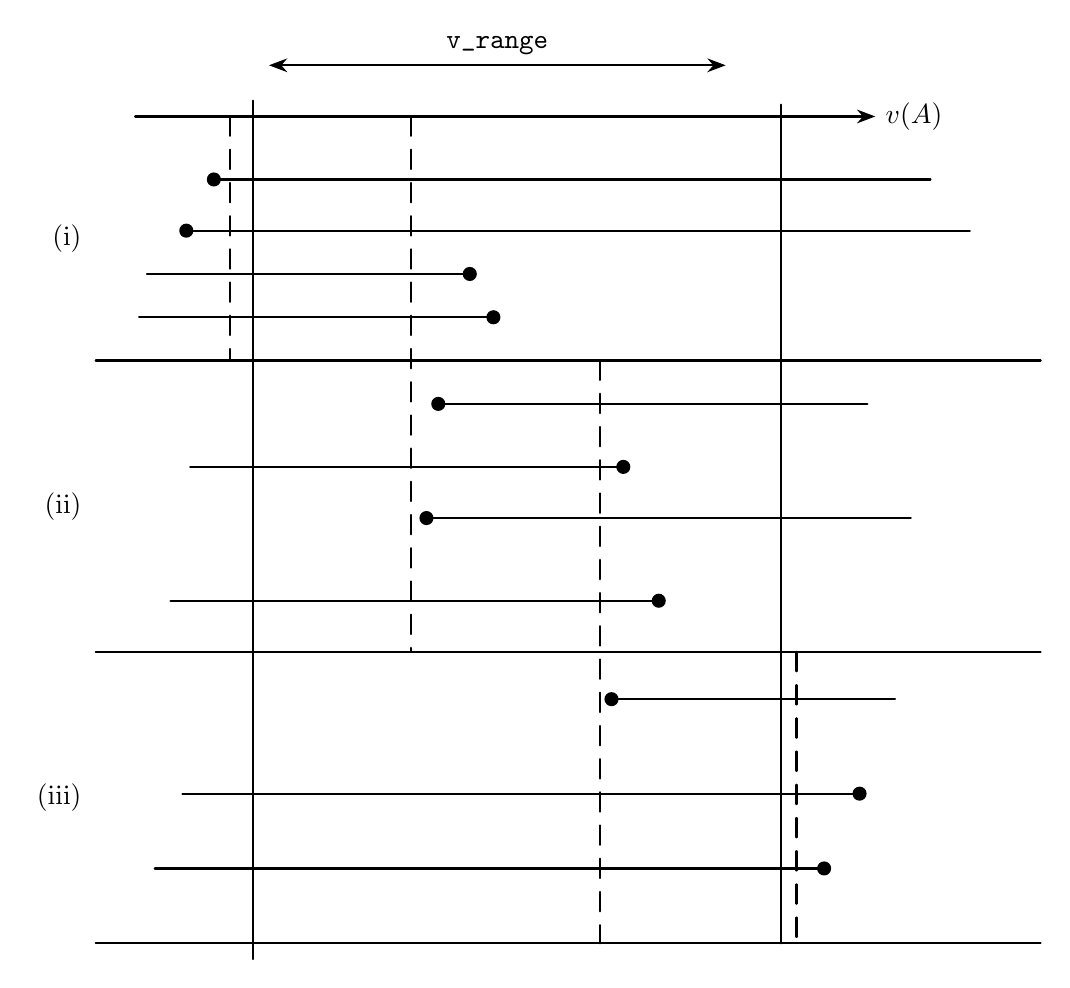
\begin{tikzpicture}[
  x=1cm,y=1cm,
  line width=0.8pt,
  line cap=round,
  guide/.style={dash pattern=on 7pt off 5pt},
  dot/.style={circle,fill=black,inner sep=1.8pt},
  >=Stealth
]
  \def\axislabel{v}

  % Horizontal axis and range annotation.
  \draw[->] (0,0) -- (9.4,0) node[right] {$v(A)$};
  \draw[<->] (1.7,0.65) -- (7.5,0.65)
    node[midway,above] {\verb|v_range|};

  % Solid vertical boundaries and horizontal panel separators.
  \draw (1.5,0.2) -- (1.5,-10.7);
  \draw (8.2,0.15) -- (8.2,-10.5);
  \foreach \y in {-3.1,-6.8,-10.5}
    \draw (-0.5,\y) -- (11.5,\y);

  % Dashed guides, with different ranges in each panel.
  \draw[guide] (1.2,0) -- (1.2,-3.1);
  \draw[guide] (3.5,0) -- (3.5,-6.8);
  \draw[guide] (5.9,-3.1) -- (5.9,-10.5);
  \draw[guide] (8.4,-6.8) -- (8.4,-10.5);

  \node[left] at (-0.55,-1.55) {\textnormal{(i)}};
  \node[left] at (-0.55,-4.95) {\textnormal{(ii)}};
  \node[left] at (-0.55,-8.65) {\textnormal{(iii)}};

  % (i): two left endpoints, followed by two right endpoints.
  \draw (1.0,-0.8) node[dot] {} -- (10.1,-0.8);
  \draw (0.65,-1.45) node[dot] {} -- (10.6,-1.45);
  \draw (0.15,-2.0) -- (4.25,-2.0) node[dot] {};
  \draw (0.05,-2.55) -- (4.55,-2.55) node[dot] {};

  % (ii): alternating left and right endpoints.
  \draw (3.85,-3.65) node[dot] {} -- (9.3,-3.65);
  \draw (0.7,-4.45) -- (6.2,-4.45) node[dot] {};
  \draw (3.7,-5.1) node[dot] {} -- (9.85,-5.1);
  \draw (0.45,-6.15) -- (6.65,-6.15) node[dot] {};

  % (iii): one left endpoint and two right endpoints.
  \draw (6.05,-7.4) node[dot] {} -- (9.65,-7.4);
  \draw (0.6,-8.6) -- (9.2,-8.6) node[dot] {};
  \draw (0.25,-9.55) -- (8.75,-9.55) node[dot] {};
\end{tikzpicture}

\end{center}

この図は，上記の計算を行った結果を，三つの\verb|case|を含むある\verb|case_family|について，
ある特定の$c^-, c_+$において図示したものである．

上記の計算により，各\verb|case|について，$v(A)$の範囲を制限する不等式がいくつか得られるが，
それらの不等式で許される$v(A)$の範囲を黒丸と半直線で表している．

また，縦の点線は，$c^-, c_+$を動かしたときのそれらの下限や上限を表している．

具体的には，一番左の点線は(i)について計算をしたとき得られる下限の，$c^-, c_+$を動かしたときの上限，
その次の点線は(i)について計算をしたとき得られる$v(A)$の範囲の上限の下限，
その次の点線は(ii)について計算をしたとき得られる上限の下限，
最後の点線は(iii)について計算をしたとき得られる上限の下限
を表している．

したがって，特定の$c^-, c_+$において図示したこの図では，
例えば(i)の計算で下限を定める黒丸（半直線が右に伸びているもの）は，すべて最初の点線より左にある．

また，(i)で上限を定める黒丸よりも，(ii)で下限を定める黒丸の方が左に描かれている，そして
また，(ii)で上限を定める黒丸よりも，(iii)で下限を定める黒丸の方が左に描かれているのは，
2番目以降の\verb|case|の計算で追加された計算によって検証されたことを表している．

この状況において，\verb|v_range|で指定された範囲に$v(A)$があるとき，(i), (ii), (iii) のいずれかの\verb|case|
の後継がすべて許容的で，かつその和集合が連結であることが分かる．

\begin{comment}
  実際，$A \in \mathcal{B}_{h,k}$を固定し，\verb|v_range|で指定された範囲に$v(A)$があるとき，そこに縦線を引くと，
どれかの\verb|case|に属する半直線とは全て交わることがわかる．
\end{comment}

一般の場合について考えよう．
\verb|case| (k)についての計算をしたときに得られる$v(A)$の範囲の上限の，$c^-, c_+$を動かしたときの下限を$M_k$とする．
すると，ある$j$があって，$M_1, \cdots, M_{j-1} \le v(A)$で$v(A) \le M_j$となる．
このとき，(i), (ii), \dots, (j)に属する黒丸と半直線たちは，$A$によって実際に指定される$s,r$をカバーしている．

そして，各$c^-, c_+$ごとに，つまり各$A$について，
各\verb|case|の連結性についての計算から得られる$v(A)$の範囲は空にならず，また，それら区間の下端は
前の\verb|case|についての計算から得られる$v(A)$の範囲の上端よりも小さくなる．つまりそれらの範囲は連結である．
そして，(i)の範囲の下端は\verb|v_range|の下端より小さく，(j)の範囲の上端は$M_j$より，したがって$v(A)$より大きい．
よって，(i), (ii), \dots, (j)のうち，どれかの\verb|case|では，それに含まれる後継の和集合が連結になることが分かる．

そして，その\verb|case|(k)について，上記の手順で計算した，含まれる後継が許容的になるのに充分な$v(A)$の範囲の下端は
$M_{k - 1}$以下，したがって$v(A)$以下であり（$k=1$なら\verb|v_range|の下端以下），上端は\verb|v_range|の上限以上
（$k=1$なら2番目の\verb|case|の計算から得られる下限以上であり，
もし$v(A)$が範囲外にあるなら，2番目以降のどれかの\verb|case|の計算から得られる範囲にもその$v(A)$は含まれる）であるから，
その\verb|case|に含まれる後継は全て許容的である．

以上より，補題\ref{Lem2}が検証できたことになる．

\begin{thebibliography}{99}
\raggedright
\bibitem{schecker} 
H. Schecker, 
{\it \"Uber die Menge der Zahlen, die als Minima quadratischer Formen auftreten}, 
J. Number Theory {\bf 9} (1977), no.~1, 121--141;

\bibitem{hall}
M.~Hall, Jr.,
\textit{On the sum and product of continued fractions},
Annals of Mathematics \textbf{48} (1947), no.~4, 966--993.
\end{thebibliography}

\end{document}
